\documentclass[conference]{IEEEtran}

\usepackage{algorithm,algorithmic}
\usepackage{graphicx}
\usepackage{color}
\usepackage{amsmath}
\usepackage{amssymb}
% Note that the amsmath package sets \interdisplaylinepenalty to 10000
% thus preventing page breaks from occurring within multiline equations. Use:
\interdisplaylinepenalty=2500
% after loading amsmath to restore such page breaks as IEEEtran.cls normally
% does.

% correct bad hyphenation here
\hyphenation{op-tical net-works semi-conduc-tor}

% command for rating prediction
\newcommand{\predr}[1]{\hat{r}_{#1}}
% command for aggregate
\newcommand{\aggr}[1]{\underset{#1}{\operatorname{aggr}}\;}
\usepackage{booktabs}

\begin{document}
%
% paper title
% Titles are generally capitalized except for words such as a, an, and, as,
% at, but, by, for, in, nor, of, on, or, the, to and up, which are usually
% not capitalized unless they are the first or last word of the title.
% Linebreaks \\ can be used within to get better formatting as desired.
% Do not put math or special symbols in the title.
\title{Analogy in Recommendation.\\ Numerical vs. Ordinal: a Discussion}


% author names and affiliations
% use a multiple column layout for up to three different
% affiliations
%\author{\IEEEauthorblockN{Nicolas Hug}
%\IEEEauthorblockA{School of Electrical and\\Computer Engineering\\
%Georgia Institute of Technology\\
%Atlanta, Georgia 30332--0250\\
%Email: http://www.michaelshell.org/contact.html}
%\and
%\IEEEauthorblockN{Henri Prade}
%\IEEEauthorblockA{Twentieth Century Fox\\
%Springfield, USA\\
%Email: homer@thesimpsons.com}
%\and
%\IEEEauthorblockN{Gilles Richard}
%\IEEEauthorblockA{Starfleet Academy\\
%San Francisco, California 96678--2391\\
%Telephone: (800) 555--1212\\
%Fax: (888) 555--1212}
%\and
%\IEEEauthorblockN{Mathieu Serrurier}
%\IEEEauthorblockA{Starfleet Academy\\
%San Francisco, California 96678--2391\\
%Telephone: (800) 555--1212\\
%Fax: (888) 555--1212}}

% conference papers do not typically use \thanks and this command
% is locked out in conference mode. If really needed, such as for
% the acknowledgment of grants, issue a \IEEEoverridecommandlockouts
% after \documentclass

% for over three affiliations, or if they all won't fit within the width
% of the page, use this alternative format:
%
\author{\IEEEauthorblockN{Nicolas Hug\IEEEauthorrefmark{1},
Henri Prade\IEEEauthorrefmark{1}\IEEEauthorrefmark{2},
Gilles Richard\IEEEauthorrefmark{1},
Mathieu Serrurier\IEEEauthorrefmark{1}}
\IEEEauthorblockA{\IEEEauthorrefmark{1}Institut de Recherche en Informatique de
  Toulouse,\\
CNRS, Universit\'e Paul Sabatier, France\\
\IEEEauthorrefmark{2} QCIS, University of Technology, Sydney, Australia
\\ Email: \{nicolas.hug, henri.prade, gilles.richard,
mathieu.serrurier\}@irit.fr}}




% use for special paper notices
%\IEEEspecialpapernotice{(Invited Paper)}




% make the title area
\maketitle

% As a general rule, do not put math, special symbols or citations
% in the abstract
\begin{abstract}
The paper investigates the use of analogical reasoning for recommendation
purposes. More particularly, we address the problem of predicting
missing ratings on the basis of known ones. After
discussing the differences with another recently experimented approach based on
analogical proportions, a new analogical approach is proposed. It relies on
the intuition that ``\textit{the rating of user $u$ for item $i$ is to the
  rating of user $v$ for item $i$ as the rating of user $u$ for item $j$ is to
the rating of user $v$ for item $j$}''.  This leads to algorithms yielding
results close to the ones of state-of-the art approaches, when the ratings are
regarded as numerical quantities. This is due to the fact that these latter
approaches embed an estimation process that is 
implicitly close to analogy, as discussed in this paper.
%turn out to be basically equivalent, formally speaking, to the
%proposed approach, although they do not refer to analogy at all. 
An analogical
approach is also outlined and briefly discussed when the ratings are
supposed to have an ordinal meaning only.
\end{abstract}





% For peer review papers, you can put extra information on the cover
% page as needed:
% \ifCLASSOPTIONpeerreview
% \begin{center} \bfseries EDICS Category: 3-BBND \end{center}
% \fi
%
% For peerreview papers, this IEEEtran command inserts a page break and
% creates the second title. It will be ignored for other modes.
\IEEEpeerreviewmaketitle



\section{Introduction}
Recommendation may refer to a variety of problems depending on the information
available. One may  try to propose items or products on the basis of their
descriptions to users whose preferences profiles are known.  One may also
take advantage of the  behavior of other users that are similar to the
recommendee. One may also  try
to predict missing ratings on the basis of  known ratings.
%only know ratings given by users to products and
 Exploiting preferences may call for fuzzy set
methods; see, e.g. \cite{Perny}, for an early example. Similarity is also a
graded notion that underlies case-based reasoning, which can be embedded in a
fuzzy rule-based approach and be related to k-nearest neighbor approaches
\cite{DHP02,HDP02,DHP06}.

The recommendation problem considered in this paper is the prediction of
missing ratings on the basis of known ratings. We more particularly explore the
idea of applying analogical reasoning to this problem.
Analogy is used here in terms of analogical proportions, i.e., statements of
the form ``$a$ is to $b$ as $c$ is to $d$''. In case-based reasoning,
situations with known conclusions are put in parallel one by one, with a new pair (situation $0$,
conclusion $0$) where `conclusion $0$' is unknown. Then case-based reasoning
can be viewed as a particular instance of analogical reasoning since one
can say that ``conclusion $0$ should be to conclusion $i$ as situation $0$ is
to situation $i$''. However there is a more sophisticated way to apply analogy
here, namely to state  that ``(situation $0$, conclusion $0$) is to (situation
$3$, conclusion $3$) as (situation $2$, conclusion $2$) is to (situation $1$,
conclusion $1$)'', which requires to put the situation on which one wants to
conclude in parallel with three other situations where the corresponding
conclusion is known \cite{DPRManta}. Then using a formal model of an analogical
proportion \cite{MicPraNAFIPS2008,PraRicLU2013}, and observing that analogical
proportions hold on various features describing the four situations, one
conclude that ``conclusion $1$ is to conclusion $2$ as conclusion $3$ is to
conclusion $0$'' should hold as well, which leads to compute `conclusion $0$'
from this latter relation.

The idea of applying analogy to recommendation is not entirely new. Thus,
Sakaguchi et al. \cite{Takagi2011} use four-terms analogy in a case-based reasoning
style for proposing dishes to users, while three of the authors of the present
paper have more recently proposed a  4-(situation, conclusion)-based analogical
mechanism for predicting missing ratings on the basis of known ratings
\cite{HugPR15}. This latter work yielded reasonably good results, but was
extremely heavy computationally speaking. In this paper, we investigate a
more tractable way of using analogical proportions for solving the same
problem. Namely, letting $r_{ui}$ be the rating for item $i$ by user $u$, we
assume that ``$r_{ui}$ is to $r_{vi}$ as $r_{uj}$ is to $r_{vj}$’’, where
$r_{vj}$ is unknown, while the three other ratings are available. We shall first
consider the ratings as numbers, which leads to an estimation process quite close
to the one used in Takagi-Sugeno fuzzy rule-based controllers \cite{TS85} where
similarity-based weighted averages are performed. We then more briefly discuss
the case where the ratings are only considered as having an ordinal meaning.

The paper is structured as follows. The next section provides the necessary
background on the modelling of analogical proportions when features are Boolean
and when they are numerical. Section 3 first recalls the previously proposed
analogical approach to the prediction of missing ratings which uses the
sophisticated mechanism involving four parallel vectors of the (situation,
conclusion)-type. Then Section 3 introduces the way analogy is applied in this
paper. Section 4 presents the algorithm that exploits this view and reports
results of experiments on the Movielens benchmark when the ratings are regarded as
numerical quantities. These results are quite close to the ones obtained by
state-of-the art approaches. This is due to the fact that the proposed
analogical approach appear to be formally very close to the state-of-the art
approaches, although the latter do not refer to analogy at all, as revealed by
the discussion ending the section.  Section 5 outlines an ordinal counterpart
to the proposed analogical approach, since it is arguable that ratings have
often mainly an ordinal meaning.

\section{Analogical reasoning with proportions}
The following section provides the necessary background on analogical
reasoning that will be used throughout this paper.

\subsection{Formal definitions}
An analogical proportion ``$a$ is to $b$ as $c$ is to $d$'' states analogical
relations between the pairs $(a,b)$ and $(c,d)$, as well as between the pairs
$(a,c)$ and $(b,d)$.  There are numerous examples of such statements, with
which everybody will more or less agree, such as  ``calf is to cow as foal is
to mare'', or ``brush is to painter as chalk is to teacher''. However, it is
only rather recently that formal definitions have been proposed for analogical
proportions, in different settings
\cite{StroppaYvon2006,LepageHDR2003,MicPraECSQARU2009}.
For more details, see \cite{PraRicLU2013,PraRicECSQARU2013,PraRicIFCOLOG2014}.

It has been agreed since Aristotle time, taking lesson from geometrical proportions, that an analogical proportion $T$, as
a quaternary relation, satisfies the three following characteristic properties:
\begin{enumerate}
\item $T(a,b,a,b)$ (reflexivity)
\item $T(a,b,c,d) \implies T(c,d,a,b)$ (symmetry)
\item $T(a,b,c,d) \implies T(a,c,b,d)$ (central permutation)
\end{enumerate}
There are various models of analogical proportions, depending on the target
domain.  When the underlying domain is fixed, $T(a,b,c,d)$ is simply denoted
$a:b::c:d$. Standard examples are:
\begin{itemize}
\item Domain $\mathbb{R}$: $a:b::c:d \text{ iff } a-b= c-d \text{ iff } a + d=
  b + c$ (arithmetic proportion)
\item Domain $\mathbb{R}^n$:
$\vec{a}:\vec{b}::\vec{c}:\vec{d} \mbox{ iff } \vec{a}-\vec{b} =
\vec{c}-\vec{d}$. This is just the extension of arithmetic proportion to real
vectors. In that case, the 4 vectors $\vec{a}, \vec{b}, \vec{c}, \vec{d}$ build
up a parallelogram.
\item Boolean domain $\mathbb{B}=\{0,1\}$:\\ $a:b::c:d \text{ iff } (a \wedge d \equiv b
  \wedge c) \wedge (a \vee d \equiv b \vee c)$
\end{itemize}

In the following, we will be mostly interested in the arithmetic proportions
in $\mathbb{R}$ or in $\mathbb{R}^n$, and will work with analogies between
ratings.

\subsection{Using analogical proportion for inference}
\label{ANALOGY_INFERENCE}
To understand how one can infer new information on the basis of analogical
proportions, we need to define the equation solving process. The equation
solving problem amounts to finding a fourth element x to make the incompletely
stated proportion $a : b :: c : x$ to hold. As expected, the solution of this
problem depends on the target model. For instance, in the case of extended
arithmetic proportions, the solution always exists and is unique: $x = b - a +
c$. In terms of geometry, this simply tells us that given 3 points, we can
always find a fourth one (aligned with, or in the same plan as a, b, c) to
build a parallelogram.

The analogical inference principle is, logically speaking, an unsound inference principle, but providing plausible conclusions \cite{PradeR10}.
It postulates that, given 4 vectors
$\vec{a},\vec{b},\vec{c}, \vec{d}$
such that the proportion holds  on some components, then it should also hold on the
remaining ones.  This can be stated as (where $\vec{a} = (a_1, a_2, \cdots
a_n)$, and $J \subset [1,n]$): $$\frac{\forall j \in J,
a_j:b_j::c_j:d_j}{\forall i \in [1,n] \setminus J, a_i:b_i::c_i:d_i} \quad
(analogical ~ inference)$$
\noindent
This principle leads to a prediction rule in the following context:
\begin{itemize}
\item 4 vectors $\vec{a},\vec{b},\vec{c},
\vec{d}$ are given where $\vec{d}$ is partially known: only the
components of $\vec{d}$ with indexes in $J$ are known.
\item Using analogical inference, we can
predict the missing components of $\vec{d}$ by solving (w.r.t. $d_i$) the set of
equations (in the case they are solvable): $$\forall i \in [1,n]
\setminus J, \quad a_i:b_i::c_i:d_i.$$
\end{itemize}
In the case where the items are such that their last component is a label,
applying this principle to a new element $\vec{d}$ whose label is
unknown leads to predict a candidate label for $\vec{d}$.

This prediction technique has been successfully applied to classification
problems in both Boolean \cite{BayMicDel2007} and numerical settings \cite{PraRicYaoIJCISIM2012}, 
thus suggesting promising results
in the recommendation task.

\section{Analogy and the recommendation problem}
This section provides some necessary background on the recommendation task, and
explores various ideas that can be developed to build an analogical
reasoning-based recommender system.

\subsection{Recommendation as prediction of missing ratings}
Let us formalize the problem of recommendation.
Let $U$ be a set of users and $I$ a set of items. For some pairs $(u,i) \in U
\times I$, a rating  $r_{ui}$ is supposed to have been given by $u$ to express
if he/she likes or not the item $i$. $R$ denotes the set of all known ratings.
Let $U_i$ be the set of users that have rated item $i$, and $I_u$ is the set of
items that user $u$ has rated. $I_{uv}$ defines the set of items rated by both
users $u$ and $v$. The ultimate goal of a recommender system is to provide
relevant and personalized recommendations of items to users, and this is
usually done by trying to predict users' ratings for any item in the the
system. Note that users and items can play symmetrical roles: indeed, one can see the recommendation problem as recommending items to users or as recommending users to items. In the following, we chose the first view which we find more intuitive for the reader.

The two main families of recommender systems are \textit{content-based} methods
where some meta data describing users and items are used, and
\textit{collaborative filtering} methods, much more popular, where predictions
are computed by taking into account the \textit{social environment} of users
which is usually modeled by the ratings they gave. Collaborative techniques are
the one we are interested in here, as they have shown to outperform the
content-based ones.

It is quite common that ratings belong to $[0, 1]$ or to $[1, 5]$, while $1$ is
the worst rating and $5$ meaning a strong preference. It is not always clear
whether this rating scale should be interpreted as purely numerical, or more
like an ordinal scale when it comes to develop prediction algorithms. This is
a question that we will address throughout this paper.

 When ratings are treated as numerical quantities, the two most used
 performance evaluation metrics are MAE (Mean Absolute Error) and RMSE (Root
 Mean Squared Error), and are usually computed using cross validation:
\begin{align}
\text{MAE} &= \frac{1}{|R|} \cdot \sum_{r_{ui}} |\predr{ui} - r_{ui}|\\
\text{RMSE} &= \sqrt{\frac{1}{|R|} \cdot \sum_{r_{ui}} (\predr{ui} - r_{ui})^2}
\end{align}
They both evaluate how close predictions are from their true values, RMSE being
much more penalizing over big errors.

\subsection{Analogical proportions between users}
\label{ANALOGY_USERS}
Using analogical reasoning for recommendation as been studied in
\cite{HugPR15}. Authors strictly follow the analogical inference
principle described in section \ref{ANALOGY_INFERENCE} for making predictions,
using analogical proportions between users.

The main idea is that if an analogical proportion stands between four users $a,
b, c, d$, meaning that for each item $j$ that they have commonly rated, the
analogical proportion $r_{aj} : r_{bj} :: r_{cj} : r_{dj}$ holds, then it
should also hold for an item $i$ that $a, b, c$ have rated but $d$ has not
(i.e. $r_{di}$ is the missing component). This leads us to estimate $r_{di}$ as
the solution $x = \predr{di}$ of the following analogical equation:
$$r_{ai} : r_{bi} :: r_{ci} : x.$$
\noindent
Given a pair $(u,i)$ such that $r_{ui} \notin R$ (i.e. there is no available
rating from user $u$ for item $i$), the main procedure is as follows:
\begin{enumerate}
\item find the set of 3-tuples of users $a, b, c$ such that an analogical
  proportion stands between $a, b, c,$ and $u$ and such that the equation
  $r_{ai} : r_{bi} :: r_{ci} : x$ is solvable.
\item solve the equation $r_{ai} : r_{bi} :: r_{ci} : x$ and consider the
solution $x$ as a candidate rating for $r_{ui}$.  \item set $\predr{ui}$ as an
  aggregate of all candidate ratings.
\end{enumerate}

This technique has shown to be not too far from basic collaborative filtering
approaches \cite{HugPR15}, but suffers of its inherent cubic complexity which makes it
impossible to look for every possible 3-tuples of users, thus compromising the
prediction accuracy.

\subsection{Pairwise analogy between clones}
Considering analogy between four users has shown to be computationally
intensive, thus not really suitable for recommendation purposes, where time is
a highly critical dimension. Yet, other forms of analogy can be addressed in
the recommendation task, based on the observation that some users may be more
inclined to give good (or bad) ratings than others. Indeed, ratings are in no
way absolute and greatly depend on the subjective appreciation each user has
about the rating scale. In the $[1, 5]$ scale for example, two users $u$ and
$v$ might semantically agree on an item $i$ describing it as $bad$, but there
is a chance that this agreement is not perfectly reflected in the ratings: $u$
might have rated $i$ with $r_{ui} = 1$ and $v$ with $r_{vi} = 3$, simply
because from $v$' point of view $3$ is a \textit{bad} rating, while for $u$ a
rating of $3$ would simply mean \textit{decent} or \textit{good enough}.  In
the following, we refer such users that \textit{semantically} agree on their
common items (but not necessarily \textit{numerically}) as \textit{clones}, as
illustrated in Figure \ref{FIG_CLONES}. Please note that the word $clone$ is
not used here to mean \textit{strictly identical}, but more in the sense that
two clones are two users following parallel paths.

\begin{figure}[!h]
\centering
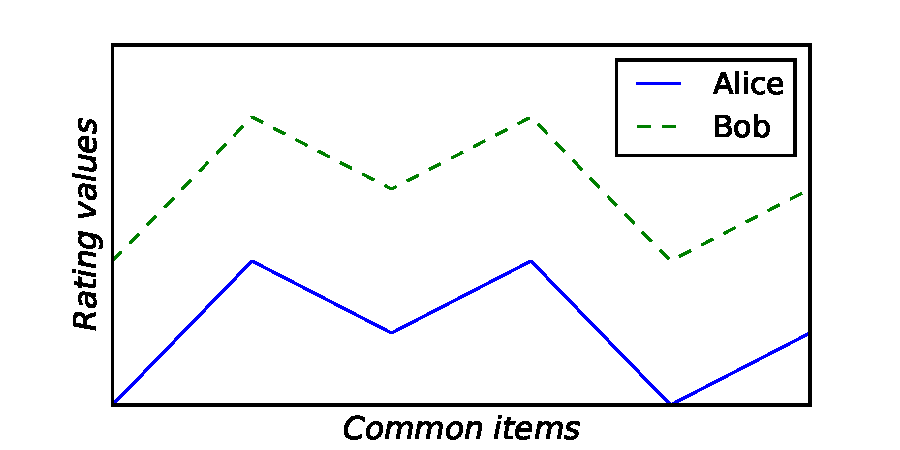
\includegraphics[width=2.5in]{clones.pdf}
\caption{Bob is a perfect clone of Alice.}
\label{FIG_CLONES}
\end{figure}

It is obvious that in collaborative filtering, clones are of great interest when
it comes to predict a user's ratings, and yet the information they provide is
often discarded.  The principle underlying the analogical clone-based view is
the following: for predicting a missing rating for $u$ we not only look at its
nearest neighbors, but also to those $v$ whose rating are such that $r_{ui} =
r_{vi} + t_{vu}$ where $t_{vu}$ is a more or less constant \textit{correction
term} that can be either positive or negative.

In the next two sections, we investigate this idea of a clone-based prediction,
first when ratings are viewed as numerical quantities in section
\ref{NUMERICAL_POV}, and then when they have an ordinal meaning only in
section \ref{ORDINAL_POV}.

\section{Ratings as numerical quantities}
\label{NUMERICAL_POV}

In the following, we define $C_i(u)$ as the set of users that are clones of $u$
and that have rated item $i$.  From the previous definitions, one can easily
derive a very general collaborative filtering framework for predicting a user's
rating by taking into account its clones:
$$\predr{ui} = \text{aggregation}(r_{vi} + t_{vu}), \quad \forall v \in
C_i(u),$$
where $t_{vu}$ is a \textit{correction term} that we need to add to $v$'s
ratings so that they correspond to those of $u$. We clearly have a
generalization of the $k$-NN approach, which we could write as:
$$\predr{ui} = \text{aggregation}(r_{vi} + t_{vu}), \quad \forall v \in \{v \in C_i(u)
  | t_{vu} = 0\}.$$

Following this general framework, one can construct a great variety of
algorithms with various level of complexity. In the next subsections, we
propose a very straightforward algorithm, and a more efficient one.

\subsection{A straightforward prediction algorithm}
\label{STRAIGHTFORWARD}

In its most simple form, a user $v$ can be considered to be a $t$-clone of $u$ if
the ratings of $v$ differ from those of $u$ from a constant $t$:
\begin{equation}
v \in t\text{-}C(u) \iff \forall i \in I_{uv}, r_{ui} = r_{vi} + t.
\end{equation}
From then on, computing $\predr{ui}$ amounts to finding all the users $v$ that
satisfy this criteria, and computing an aggregation of their rating for $i$,
which can simply be a mean. We implemented this basic algorithm described by
algorithm \ref{algo_straight}, and referred to as \textit{Bruteforce}.

 \begin{algorithm}[!ht]
   \caption{\textit{Bruteforce}}
       \label{algo_straight}
       \begin{algorithmic}

      \STATE {\bf Input}: A set of known ratings $R$, a user $u$, an item
      $i$ such that $r_{ui} \notin R$.
      \STATE {\bf Output}: $\hat{r}_{ui}$, an estimation of $r_{ui}$

      \STATE {\bf Init}:
      \STATE $C = \varnothing$ \quad \quad // list of candidate ratings
      \FORALL{ users $v \in U_i$}
        \FORALL{$t$}
          \IF{$v \in t\text{-Clones}(u)$}
          \STATE $C \gets C \cup \{r_{vi} + t\}$ \quad // add x as a candidate rating
          \ENDIF
        \ENDFOR
	    \ENDFOR
    \STATE $\hat{r}_{ui} = \aggr{x \in C} x$
\end{algorithmic}
\end{algorithm}

Of course, one may want to relax the definition of a $t$-clone, as the current
one is too strict and only very few users will satisfy this criteria. In our
implementation, we chose the following condition:
$$v \in t\text{-}C(u) \iff \sum_{i \in I_{uv}} |(r_{ui} - r_{vi}) - t| \leq |I_{uv}|.$$
This amounts to accept $v$ as a $t$-clone of $u$ if on average, $r_{ui} -
r_{vi}$ is equal to $t$ with a margin of $1$.

The values of $t$ clearly depend on the rating scale. The dataset on which we
tested our algorithms use the $[1, 5]$ interval, so possible values for $t$
that were considered are integer values between $[-4, 4]$.

This is obviously a very rough algorithm, to which one could point out numerous
flaws, but its purpose is to show that even such a basic clone-based approach
can lead to better results than a basic neighborhood method.

\subsection{Modeling clones with the similarity measure}
\label{MODELING_CLONES}
Another option to consider clones is to use the well known neighborhood-based
formula, and capture their effect inside an appropriate similarity measure. The
general neighborhood formula is as follows \cite{handbookRecoSys2011}:

$$\predr{ui} = \frac{\sum_{v \in N_i^k(u)} r_{vi} \cdot sim(u, v)}{\sum_{v \in
  N_i^k(u)} sim(u, v)},$$
where $N_i^k(u)$ is the set of the $k$ nearest neighbors of $u$ that have rated
$i$. So, we move from a crisp view of the set of clones to a fuzzy one. In fact, the above formula looks very similar to the interpolation principle underlying Takagi-Sugeno fuzzy controller where similarity degree is viewed as a fuzzy membership grade \cite{TS85}.

The above formula is commonly used with classical similarity metrics such as
Pearson or cosine similarity, or inverse of MSD (Mean Squared Difference, which is
a distance).
However, these similarities are not plainly satisfactory when it comes to
clones. Indeed with these metrics, two users are considered to be close if
their common ratings are often the same, but two perfect clones $u$ and $v$
with a significant correction term $t_{vu}$ would be considered as far from
each other, thus involving a loss of information.

A simple choice to measure how two users relate as clones can be the following:
$$Clone\_dist(u, v) =  \frac{1}{|I_{uv}|} \cdot \sum\limits_{i \in I_{uv}}
((r_{ui} - r_{vi}) - \mu_{uv})^2$$
where $\mu_{vu}$ is the mean difference between ratings of $u$ and $v$:
$$\mu_{uv}= \frac{1}{|I_{uv}|}\sum_{i \in I_{uv}} (r_{ui} - r_{vi}).$$

One can understand this distance in two ways:
\begin{itemize}
\item it can be regarded as the variance of the difference of ratings between
  $u$ and $v$,
\item or it can be regarded as a simple MSD measure ($\text{MSD}(u, v) =
  \frac{1}{|I_{uv}|} \cdot \sum\limits_{i \in I_{uv}}
  (r_{ui} - r_{vi})^2$)
 to which the mean difference of ratings between $u$ and $v$ has been
 subtracted.
  \end{itemize}

As our measure $Clone\_dist$ is a distance, it is necessary to transform it
into a similarity measure. Common choice is to take its inverse (while accounting for zero division): $Clone\_sim(u,
v) = \frac{1}{Clone\_dist(u, v) + 1}$.

Once we know how to find the clones of a user, it is a simple matter to output
a prediction using the classical neighborhood approach:
$$\predr{ui} = \frac{\sum_{v \in N_i^k(u)} (r_{vi} + \mu_{uv}) \cdot sim\_clone(u,
v)}{\sum_{v \in N_i^k(u)} sim\_clone(u, v)}.$$

This algorithm will be referred to as $CloneA$. For the sake of completeness,
we also tried the same formula but with a more basic similarity metric that
does not care about clones: MSD. This algorithm is referred to as $CloneB$.

\subsection{Current practices in neighborhood-based methods}

A simple and efficient formula using neighborhood technique, popularized by
\cite{Koren:2010:FNS:1644873.1644874} is the following:
$$\predr{ui} = b_{ui} + \frac{\sum_{v \in N_i^k(u)} (r_{vi} - b_{vi}) \cdot
sim(u, v)} {\sum_{v \in N_i^k(u)}sim(u, v)}.$$
It is based on a simple $k$-NN approach, where are added the $b_{ui}$ terms,
called \textit{baselines}: $b_{ui} = \mu + b_u + b_i$. $\mu$ is the global mean
of all ratings in $R$. The $b_u$ term is intended to capture users propensity
to give ratings higher or lower than the global mean $\mu$, and the same goes
for items with $b_i$: some items tend to be rated higher than others. Baselines
are computed by solving a least squares problem:
$$ \min\limits_{b_u, b_i} \sum_{r_{ui} \in R} (r_{ui} - (\mu + b_u + b_i))^2,$$
which can be achieved efficiently by stochastic gradient descent, or
alternating least squares.

Among recommended similarity metrics, this one is of particular interest:
$$\text{sim}(u, v) = \frac
{ \sum\limits_{i \in I_{uv}} (r_{ui} -  b_{ui}) \cdot (r_{vi} - b_{vi})}
{\sqrt{\sum\limits_{i \in I_{uv}} (r_{ui} -  b_{ui})^2} \cdot
\sqrt{\sum\limits_{i \in I_{uv}} (r_{vi} -  b_{vi})^2}}.$$

It is simply a Pearson correlation coefficient, except that instead of
centering ratings by their means, they are centered with the baseline
predictors. An intuitive and illuminating way to look at this algorithm as a
whole is to see that it conceptually follows these steps:
\begin{enumerate}
  \item Compute $R'$, the set of all ratings normalized by the corresponding
    baseline: $r'_{ui} = r_{ui} - b_{ui}$.  $R'$ can be regarded as the set
    where all ratings are given from the same frame of reference, thus
    discarding any bias.  In $R'$, ratings can then be considered as absolute.
  \item Using $R'$, compute similarities between users using the cosine similarity (the
    cosine similarity is the same as the Pearson correlation coefficient,
    except that quantities are not centered).
  \item Output a prediction using the basic $k$-NN formula. As this prediction
    belongs to the same space of $R'$ where ratings have no bias, it needs to
    be transposed back to the space of $R$ (for performance evaluation
    purposes).
\end{enumerate}

In what follows, this algorithm is referred to as $k$-NNbsl.

It is very clear that the use of the baseline predictors is motivated by the
same reasons one would want to consider clones in a rating prediction
algorithms. This means that $k$-NNbsl implicitly takes the idea of clones into account, and thus a form of analogical reasoning.
Differences and resemblances of these two approaches are discussed
in the next section.

\subsection{Experiments and discussion}
\label{expeDiscuss}

We evaluated the performance of the aforementioned algorithms in terms of MAE
and RMSE on two datasets, the movielens-100K and movielens-1M
datasets\footnote{http://grouplens.org/datasets/movielens}, containing
$100,000$ and $1M$ ratings respectively. Results are shown in tables
\ref{table:res100k} and \ref{table:res1M} and where calculated using 5-folds
cross-validation. For each of these algorithms, the number of neighbors or
clones used to output a prediction is $k = 40$, except for the bruteforce
algorithm where the number of clones can not be controlled.
\begin{table}[!ht]
\centering
\caption{Performance of algorithms on the Movielens-100k dataset}
\label{table:res100k}
\begin{tabular}{| c || c | c | c | c | c | c |}
\toprule
     &  k-NN & Bruteforce & Clone A & Clone B & $k$-NNbsl\\
\midrule
RMSE & .9763 &   .9461    &   .9353 &  .9311  &  .9338   \\
MAE  & .7705 &   .8576    &   .7327 &  .7321  &  .7337   \\
\bottomrule
\end{tabular}
\end{table}

\begin{table}[!ht]
\centering
\caption{Performance of algorithms on the Movielens-1M dataset}
\label{table:res1M}
\begin{tabular}{| c || c | c | c | c | c | c |}
  \toprule
     &  k-NN & Bruteforce & Clone A & Clone B & $k$-NNbsl\\
  \midrule
RMSE & .9216 &           .&   .8996 &  .8969  &  .8879\\
MAE  & .7252 &           .&   .7057 &  .7050  &  .7005\\
\bottomrule
\end{tabular}
\end{table}

It is very clear that even a very straightforward approach of the clone-based
recommendation principle significantly outperforms the most basic $k$-NN
algorithm. It is however a lot heavier to compute, thus not very suitable for
real world recommendation purposes (its performances on the Movielens-1M
dataset simply could not be computed). The two other clone-based algorithms
however, have the exact same complexity of any $k$-NN-based algorithm which is
a significant improvement from the algorithm described in section
\ref{ANALOGY_USERS}.


Surprisingly enough, out of the two Clone algorithms, it is the one that does
not care about clones in its similarity measure that achieves the best results.
This might be due to the fact that in the neighborhood based on MSD, $\mu_{uv}$
is necessarily small and thus easier to estimate in a statistical significant
way.

Performances of the Clone algorithms are close to those of the state of the
art $k$-NNbsl algorithm. It is however important to understand that these
algorithms differ on the following points:
\begin{itemize}
\item The Clone algorithms do not address item bias, which is a significant
  drawback. It may not be unreasonable to believe that incorporating item bias
  in the prediction would lead to better results.
\item There is a subtle yet meaningful difference of interpretation between the
  biases induced by both algorithms. In the clone algorithm, biases are all
  pairwise, meaning that they involve two users, and they are computed on items
  that both users have rated. As for the $k$-NNbsl algorithm, there is no such
  thing as a pairwise bias. Bias for a given user is computed using only its
  own ratings, and is a result of a global optimization problem involving the
  global mean of all ratings, which means that every single rating in $R$ has
  an impact on the bias.
\item On the biggest dataset (Movielens-1M), the $k$-NNbsl algorithm appears to
  achieve better accuracy than the other algorithms, while this is not the case
  for the small dataset. A possible explanation is that as baselines are
  computed on the whole training set, they tend to capture most of the noise
  when the training set gets bigger, thus improving accuracy compared to more
  heuristic-based approach.
\end{itemize}

It should also be noted that in fact, it is recommended to perform a shrinkage
on the similarity measure of algorithm $k$-NNbsl, in order to take into account
the number of common items between two users: the more items they share, the
more confident we are when computing their similarity
\cite{Koren:2010:FNS:1644873.1644874}.
Such an approach can improve significantly both RMSE and MAE of the algorithm.
Similarly, in the clone-based approach, it might be of interest to discount
clones that rely on a too small number of common items.

\section{Towards an ordinal view of ratings}
\label{ORDINAL_POV}

We may wonder if one can devise a counterpart of the numerical clone-based approach, which would be compatible with an ordinal view of the ratings. Indeed, an extreme way for unbiasing and comparing two sets of ratings is to forget about their numerical values, and only consider their rankings.
The idea of viewing ratings in a ordinal manner has been advocated in
\cite{KorenOrdRec}.
In this section, we discuss an ordinal counterpart of the analogical approach previously presented.
Analogical reasoning with ordinal data has first been proposed in \cite{MicletBarbot09}, yet with a different concern.

\subsection{An algorithm for rank prediction}
Indeed the idea that ``\textit{the rating of user $u$ for item $i$ is to the
rating of user $v$ for item $i$ as the rating of user $u$ for item $j$ is to
the rating of user $v$ for item $j$}’’ may be understood  as well in an ordinal
manner. This leads to state that ``\textit{the relative ranking of item $i$
  among the ratings given by user $u$  is to the relative ranking of item $i$
  among the ratings given by user $v$ as the relative ranking of item $j$ among
  the ratings given by user $u$  is to the relative ranking of item $j$ among
the ratings given by user $v$}.

This means that we need to compare the rankings given by two users $u$ and $v$
on their common items. In the following, $\rho_{ui}$ denotes the relative
ranking of item $i$ out of all the items rated by $u$. Our goal is to estimate
all values of $\rho_{ui}$, for any user and any item. The main steps of a
possible algorithm is as follows:
\begin{enumerate}
  \item Compute similarities between users, based on their rankings. A very
    popular similarity ranking measure is the Spearman's rank correlation
    coefficient, or Spearman's rho.
  \item Compute an estimated rank $\hat{\rho}_{ui}$ as an aggregation of all the
    rankings $\rho_{vi}$ extracted from the $k$ nearest neighbors (using
    Spearman's rho as similarity):
    $$\hat{\rho}_{ui} = \frac{\sum_{v \in N_i^k(u)} \rho_{vi} \cdot
    sim(u, v)}{\sum_{v \in N_i^k(u)} sim(u, v)}.$$
\end{enumerate}

This is obviously very similar to the neighborhood approach described in
section \ref{MODELING_CLONES}, but instead of predicting a rating, we output a
predicted rank. This approach is denoted as \textit{RankAnlg}.


\subsection{Experiments}

We evaluated the performance of our algorithm and compared it to other
previously described approaches, using the exact same evaluation protocol as in
section \ref{expeDiscuss}. The Movielens-1m dataset was not benchmarked, as our
algorithm is too computationally intensive.

RMSE and MAE are good measure for evaluation rating prediction accuracy, but
are not suitable when it comes to evaluate rankings. A better measure is the
Fraction of Concordant Pair, which evaluates the probability that given any two
items $i$ and $j$ rated by any user $u$, the system has correctly estimated
whether $u$ prefers $i$ over $j$ or the inverse. To compute the FCP, we need to
intermediate measures. $c_u$ defines the number of concordant pairs for user
$u$, and $d_u$ its number of discordant pairs. The FCP is then computed over all
users as the proportion of concordant pairs.

\begin{align*}
&c_u = \{(i, j) \in I^2 \quad s.t. \quad \predr{ui} > \predr{uj} \text{ and }
r_{ui} > r_{uj}\}\\
&d_u = \{(i, j) \in I^2 \quad s.t. \quad \predr{ui} \geq \predr{uj} \text{ and }
r_{ui} < r_{uj}\}\\
&FCP = \frac{\sum\limits_{u \in U} c_u}{\sum\limits_{u \in U} c_u + \sum\limits_{u \in U} d_u}
\end{align*}
Note that $\predr{ui}$ here may represent either a rating prediction or a
ranking prediction $\hat{\rho_{ui}}$.

Results are reported in table \ref{table:res100kRank}.

\begin{table}[!ht]
\centering
\caption{Performance of algorithms on the Movielens-100k dataset (ranking
evaluation)}
\label{table:res100kRank}
\begin{tabular}{| c || c | c | c |}
\toprule
     & RankAnlg &  k-NN & $k$-NNbsl\\
\midrule
FCP  &  .7063   & .7096 &  .7163   \\
\bottomrule
\end{tabular}
\end{table}

Unfortunately, even a basic algorithm that was not designed for ranking
prediction performs better in terms of FCP. To explain this difference, one may
look at the distribution of average support over all the predictions, as shown
on figure \ref{FIG_SUPPORT}. Between
two users $u$ and $v$, the support is defined as the number of common items
($|I_{uv}|$), which was used to compute the similarity between $u$ and $v$. For
a given prediction $\predr{ui}$, the average support is the average of all the
supports $|I_{uv}|$ over all users $v \in N_i^k(u)$.

\begin{figure}[!h]
\centering
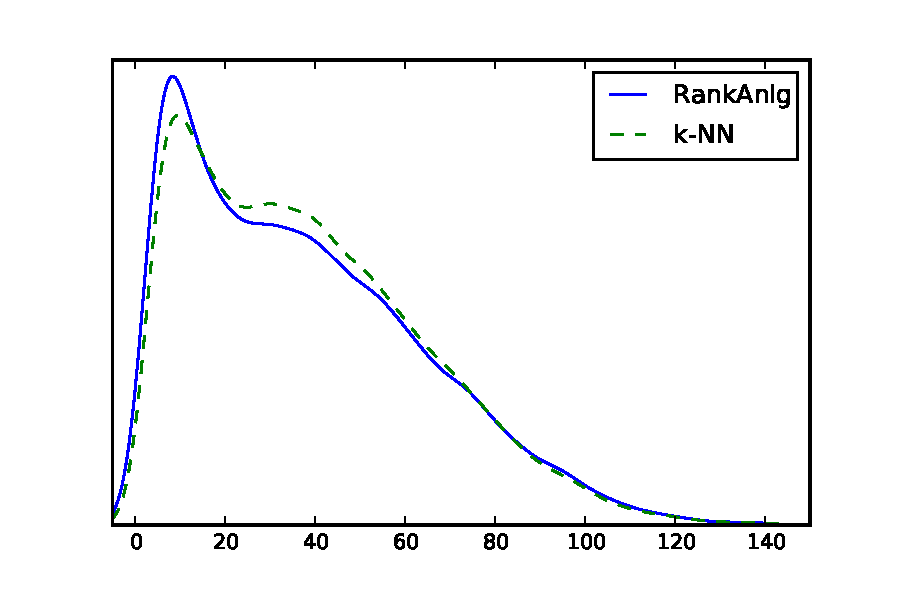
\includegraphics[width=2.5in]{support.pdf}
\caption{Distribution of average support.}
\label{FIG_SUPPORT}
\end{figure}

The use Spearman's rho tends to provide with neighbors that have smaller
support, thus leading to a less significant and less accurate estimation of the
neighborhood, which may explain the differences in performance.

\section{Conclusion}

This paper has provided a discussion on different ways for applying analogical
reasoning to the prediction of ratings.  After reporting a recent attempt where
analogical proportions were built from 4-tuples of users, a
computationally simpler approach is presented in this paper based on the idea
that ``\textit{the rating of user $u$ for item $i$ is to the rating of user $v$
  for item $i$ as the rating of user $u$ for item $j$ is to the rating of user
  $v$ for item $j$}’’.  This agrees with the transitive nature of the
  underlying analogical modeling.  We have shown that this may apply to a
  quantitative view of ratings as well as to an ordinal view.  Results obtained
  in the case of the quantitative view remain close to the ones of state-of-the
  art approaches, which can be retrospectively reinterpreted in an analogical
  way.
  
The idea behind the use of analogies is to go beyond the classical neighborhood
to extract relevant information. However, this approach has a cost as it is more difficult
to statistically validate the analogical link between users (or items).
This is especially true in the ordinal case.
Indeed, ordinal analogies tend to select users with a small common support, 
because it is easy to have the same ranking despite the fact this is not statistically relevant. 

In the specific case of MovieLens dataset, a large majority of  users seem to have  a lot of close neighbors (in the classical sense)
from which
useful information can be extracted. In that case, examples for which analogical 
links bring more information than simple neighbors are quite rare.
It should not come as a surprise that the pure analogical approach does not bring better results
than standard approaches in this dataset.

The analogical approach  might be advantageous in the case of low density 
dataset (i.e. when the set of close neighbors is small).  In the same way, we might also think of combining
the analogical approach with the classical one provided we are able to detect, for every prediction, which method
is statistically the most relevant.

Formalizing analogical reasoning provides tools for extrapolation.  This can be
done in different ways as shown in this paper, depending on what basis we try
to extrapolate. Another issue is to wonder about what we try to extrapolate.
Thus, regarding recommendation, one might think of also using analogical
reasoning to create configurations describing new items that may plausibly
please users.

%\newpage
\bibliographystyle{ieeetr}
\bibliography{biblio,biblioRecSys}

\end{document}
